%==============================================================================
% General LaTeX Report Template
%==============================================================================
% First tex file will cover the implementation of the:
% Address Decode Implementation

\documentclass[12pt]{article}

%-------------------------- Packages -----------------------------------------
\usepackage[utf8]{inputenc}       % UTF-8 encoding
\usepackage[T1]{fontenc}          % 8-bit T1 fonts
\usepackage{amsmath,amssymb}      % Math symbols
\usepackage{graphicx}             % Include graphics
\usepackage{float}                % Figure/table placement
\usepackage{hyperref}             % Hyperlinks
\usepackage{fancyhdr}             % Custom headers/footers
\usepackage{natbib}               % Bibliography
\usepackage{doi}                  % DOI links
\usepackage{listings}             % Code listings
\usepackage{xcolor}               % Colors
\usepackage{tikz}                 % Diagrams
\usepackage{pgfplots}             % Plots
\usepackage{enumitem}             % Custom lists

%----------------------- TikZ Libraries -------------------------------------
\usetikzlibrary{arrows.meta,positioning,shapes.geometric,fit,calc, matrix}
\tikzset{
  comp/.style={draw,rounded corners,thick,fill=#1!12,minimum width=28mm,minimum height=12mm},
  flow/.style={-Latex,thick},
  note/.style={font=\small\itshape,align=center}
}

%----------------------- Document Metadata -----------------------------------
\newcommand{\AuthorOne}{Mike Orduna}
\newcommand{\Class}{Digital System Design Using HDL}
\newcommand{\ReportTitle}{Processor Design Report: \\[0.5em]
  Address Decode Implementation}
\newcommand{\ShortReportTitle}{Address Decode Implementation}
\newcommand{\School}{Texas State University}

%----------------------- Coordinate Grid -----------------------------------
\newcommand{\makepcoords}[4]{% nx ny dx dy
  \foreach \i in {0,...,#1}{
    \foreach \j in {0,...,#2}{
      \coordinate (p\i\j) at (\i*#3,\j*#4);
    }
  }
}
\newcommand{\showpgrid}[4]{% nx ny dx dy
  \draw[help lines,xstep=#3,ystep=#4] (0,0) grid (#1*#3,#2*#4);
}

%---------------------- Figures and Diagrams ---------------------------------

% Figure 1: Conceptual Flow
% addr[15:0] ──► [ MSB Extract (15:12) ] ──► [ Region Decode ] ──► did
%                                   │
% rd ───────┐                       │
%           ├──► [ Access Check ] ──┴────────► hit
% wr ───────┘
\definecolor{cA}{HTML}{2E86AB} % blue - rd
\definecolor{cB}{HTML}{F18F01} % orange - wr
\definecolor{cC}{HTML}{88B04B} % green - addr
\definecolor{cD}{HTML}{E94F37} % red - hit
\definecolor{cE}{HTML}{FFC0CB} % pink - did
\definecolor{cF}{HTML}{9B30FF} % purple - MSB Extract
\definecolor{cG}{HTML}{26A69A} % teal - Access Check
\definecolor{cH}{HTML}{B2FF59} % lime - Region Decode
\newcommand{\conceptflow}{
  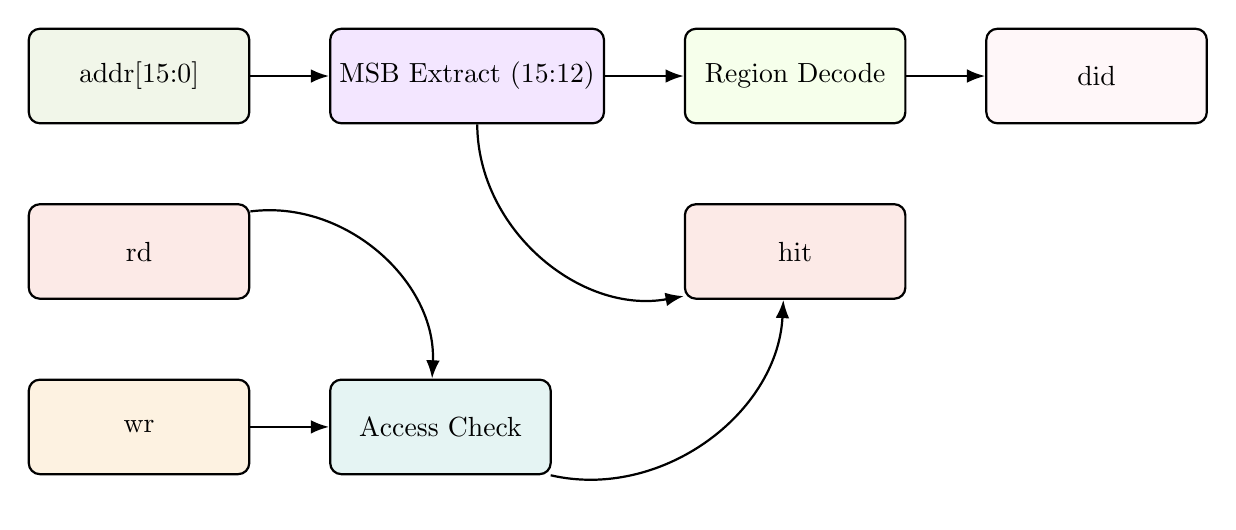
\begin{tikzpicture}[->, node distance=1cm, every state/.style={thick, minimum size=1.2cm}]
    % Nodes  
    \node[comp=cC] (addr) {addr[15:0]};
    \node[comp=cF, right=of addr] (msb) {MSB Extract (15:12)};
    \node[comp=cH, right=of msb] (dec) {Region Decode};
    \node[comp=cE, right=of dec] (did) {did};
    \node[comp=cA, below=of addr] (rd) {rd};
    \node[comp=cB, below=of rd] (wr) {wr};
    \node[comp=cG, right=of wr] (ac) {Access Check};
    \node[comp=cD, below=of dec] (hit) {hit};

    % Paths
    \draw[flow] (addr) -- (msb);
    \draw[flow] (msb) -- (dec);
    \draw[flow] (msb) to[bend right=50] (hit);
    \draw[flow] (dec) -- (did);
    \draw[flow] (rd) to[bend left=50] (ac);
    \draw[flow] (wr) -- (ac);
    \draw[flow] (ac) to[bend right=50] (hit);
  \end{tikzpicture}
}

% Figure 2: Address Space Partitioning
\definecolor{cA}{HTML}{E94F37} % red
\definecolor{cB}{HTML}{F18F01} % orange
\newcommand{\spacepartition}{
  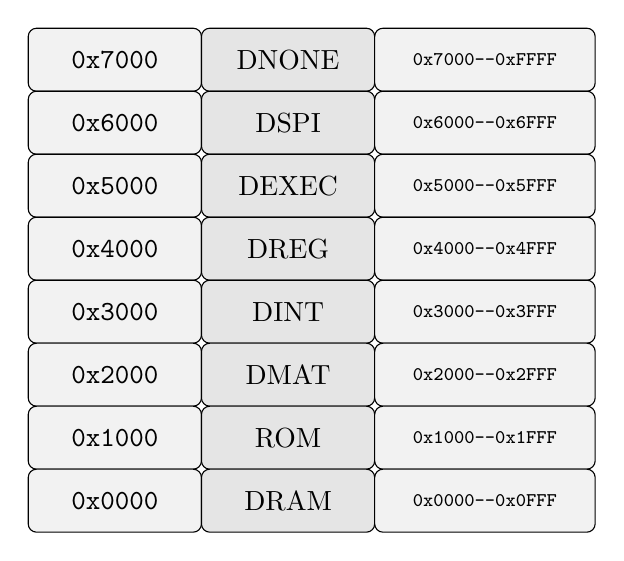
\begin{tikzpicture}[
  box/.style={draw, rounded corners=3pt, minimum height=8mm, align=center, inner sep=2pt},
  addr/.style={box, fill=black!5, font=\ttfamily, minimum width=2.2cm},
  reg/.style ={box, fill=black!10, minimum width=2.2cm},
  rng/.style ={box, fill=black!5, font=\ttfamily\scriptsize, minimum width=2.8cm},
  every node/.style={outer sep=0pt}
]
  % Left column regions (bounds)
  \node[addr] (l7) {0x7000};
  \node[addr, below=0pt of l7] (l6) {0x6000};
  \node[addr, below=0pt of l6] (l5) {0x5000};
  \node[addr, below=0pt of l5] (l4) {0x4000};
  \node[addr, below=0pt of l4] (l3) {0x3000};
  \node[addr, below=0pt of l3] (l2) {0x2000};
  \node[addr, below=0pt of l2] (l1) {0x1000};
  \node[addr, below=0pt of l1] (l0) {0x0000};

  % Middle column regions (labels)
  \node[reg, right=0pt of l7] (m7) {DNONE};
  \node[reg, below=0pt of m7] (m6) {DSPI};
  \node[reg, below=0pt of m6] (m5) {DEXEC};
  \node[reg, below=0pt of m5] (m4) {DREG};
  \node[reg, below=0pt of m4] (m3) {DINT};
  \node[reg, below=0pt of m3] (m2) {DMAT};
  \node[reg, below=0pt of m2] (m1) {ROM};
  \node[reg, below=0pt of m1] (m0) {DRAM};

  % Right column (address ranges)
  \node[rng, right=0pt of m7] (r7) {0x7000--0xFFFF};
  \node[rng, below=0pt of r7] (r6) {0x6000--0x6FFF};
  \node[rng, below=0pt of r6] (r5) {0x5000--0x5FFF};
  \node[rng, below=0pt of r5] (r4) {0x4000--0x4FFF};
  \node[rng, below=0pt of r4] (r3) {0x3000--0x3FFF};
  \node[rng, below=0pt of r3] (r2) {0x2000--0x2FFF};
  \node[rng, below=0pt of r2] (r1) {0x1000--0x1FFF};
  \node[rng, below=0pt of r1] (r0) {0x0000--0x0FFF};
\end{tikzpicture}
}


%---------------------------- Tables ------------------------------------------
\newcommand{\memorymap}{
  \begin{tabular}{|c|c|p{5cm}|}
    \hline
    \textbf{Address Range} & \textbf{Module} & \textbf{Description} \\ \hline
    0x0000-0x0FFF & Main Memory (DRAM) & Data storage for matrices and integers. \\ \hline
    0x1000-0x1FFF & Instruction Memory (ROM) & Storage for program opcodes. \\ \hline
    0x2000-0x2FFF & Matrix ALU (DMAT) & Matrix multiplication, addition, and transposition. \\ \hline
    0x3000-0x3FFF & Integer ALU (DINT) & Standard arithmetic (Add, Sub, Mul, Div). \\ \hline
    0x4000-0x4FFF & Register File (DREG) & Internal processor registers. \\ \hline
    0x5000-0x5FFF & Execution Engine (DEXEC) & Control unit for sequencing and coordination. \\ \hline
    0x6000-0x6FFF & SPI Master Module (DSPI) & External communication interface. \\ \hline
    0x7000-0xFFFF & Invalid/Unmapped (DNONE) & Ranges resulting in a \texttt{hit = 0} and \texttt{did = DNONE} state. \\ \hline
  \end{tabular}
}

\newcommand{\interface}{
  \begin{tabular}{|c|c|c|c|p{5cm}|}
    \hline
    \textbf{Signal} & \textbf{Dir.} & \textbf{Width} & \textbf{Type} & \textbf{Description} \\ \hline
    \texttt{rd}   & In  & 1  & \texttt{logic}        & Read request (active-high). \\ \hline
    \texttt{wr}   & In  & 1  & \texttt{logic}        & Write request (active-high). \\ \hline
    \texttt{addr} & In  & 16 & \texttt{logic [15:0]} & Address presented to decoder. \\ \hline
    \texttt{hit}  & Out & 1  & \texttt{logic}        & High when mapped and \texttt{rd} or \texttt{wr} asserted. \\ \hline
    \texttt{did}  & Out & 3  & \texttt{logic [2:0]}  & Device ID (valid only when \texttt{hit=1}). \\ \hline
  \end{tabular}
}

%----------------------- Header and Footer -----------------------------------
\pagestyle{fancy}
\fancyhf{}                            % clear all header/footer fields
\fancyhead[L]{\textbf{\ShortReportTitle}}
\fancyhead[R]{\today}
\fancyfoot[C]{\thepage}

%----------------------- Listings Style --------------------------------------
\definecolor{codegreen}{rgb}{0,0.6,0}
\definecolor{codegray}{rgb}{0.5,0.5,0.5}
\definecolor{codepurple}{rgb}{0.58,0,0.82}
\definecolor{backcolour}{rgb}{0.95,0.95,0.92}

\lstdefinestyle{mystyle}{
    backgroundcolor=\color{backcolour},
    commentstyle=\color{codegreen},
    keywordstyle=\color{magenta},
    numberstyle=\tiny\color{codegray},
    stringstyle=\color{codepurple},
    basicstyle=\ttfamily\footnotesize,
    breaklines=true,
    captionpos=b,
    keepspaces=true,
    numbers=left,
    numbersep=5pt,
    showspaces=false,
    showstringspaces=false,
    tabsize=2
}
\lstset{style=mystyle}

%----------------------- Hyperref Options ------------------------------------
\hypersetup{hidelinks}

%--------------------------------- Document -----------------------------------
\begin{document}

% Title Page
\begin{titlepage}
  \centering
  {\LARGE \Class}\\[2.0em]
  {\Large \ReportTitle}\\[2.0em]
  {\AuthorOne}\\[1.5em]
  {\large \School}\\[3.0em]
  {\today}
\end{titlepage}

% Table of Contents
\tableofcontents
\thispagestyle{empty}
\newpage

% Abstract
\begin{abstract}
  % Provide a brief summary of objectives, methods, and key results.
  This report documents the design and implementation of the Address Decoder
  for the Simplistic Processing Engine (SPE). The decoder serves
  as a centralized, combinational module responsible for interpreting a 16-bit
  memory-mapped address bus and identifying the targeted subsystem during read or
  write operations. By decoding the upper address bits, the module generates a
  device identification signal (\texttt{did}) and a corresponding validity signal
  (\texttt{hit}), which together coordinate access between the execution engine
  and memory-mapped functional units.

  The decoder is intentionally limited in scope: it performs no data movement,
  does not arbitrate bus ownership, and remains agnostic to downstream control
  semantics. This separation of concerns enables modular verification, minimizes
  selection latency, and prevents duplication of decode logic elsewhere in the
  processor. The report details the address space organization, decode semantics,
  interface contract, and verification strategy, while also discussing architectural
  trade-offs, growth potential, and known limitations of the current flat memory
  map approach.
\end{abstract}

% Start page numbering
\setcounter{page}{1}

%==============================================================================
% Sections
%==============================================================================

\section{Purpose and Scope}
% Introduce the purpose, scope, and structure of the report.
The address decoder is a foundational module within the Simplistic Processing
Engine or SPE. It is designed to centralize memory map logic into a single
component and prevent any duplication of decoding hardware/logic elsewhere
in the design.

\subsection{Core Functionality}
The address decoder has two primary functions:
\begin{itemize}
  \item \textbf{Address Interpretation}: The decoder interprets a 16-bit address
  bus to identify which memory-mapped device is being targeted. 
  \item \textbf{Module Selection}: The decoder generates a specific device identification
  signal—a \texttt{did}—and a validity signal—a \texttt{hit}. Both of these signals are used to coordinate
  communication between the execution engine and other functional units within the system.
\end{itemize}

\begin{figure}[H]
  \centering
  \conceptflow{}
  \caption{Combinational decode dataflow. The decoder extracts \texttt{addr[15:12]} to select a 
  mapped region (\texttt{did}) while \texttt{rd/wr} date the access request. The outputs
  \texttt{hit} and \texttt{did} are produced without state or arbitration. Downstream logic
  must act only when \texttt{hit = 1}.}
  \label{fig:conceptflow}
\end{figure}

\begin{figure}[H]
  \centering
  \spacepartition{}
  \caption{Flat 16-bit address map used by the decoder. Each \texttt{addr[15:12]} nibble selects a 
  fixed 0x1000 window (0xX000-0xXFFF) that maps to a single subsystem. All regions 0x7000-0xFFFF
  are treated as unmapped and must yield \texttt{hit = 0} with \texttt{did = DNONE}.}
  \label{fig:spacepartition}
\end{figure}


\subsection{Exclusions and Assumptions}
The decoder is strictly responsible for identification and does not handle the flow of data
movement, bus contracts, or the internal logic behind the memory-mapped modules themselves.
This separation of concerns allows for the decoder to be documented and verified independently
from the memory unit's physical implementations. Furthermore, the design assumes a 16-bit address
bus to identify which memory-mapped device is being targeted.

\section{Address Space Definition}
% Describe the address space and its organization.
The SPE utilizes a fixed 16-bit address bus width. The address space is partitioned to accommodate
main memory, instruction memory, internal registers, and specialized functional units.

\subsection{Decode Granularity}
The decoder performs device selection using the four most significant address bits, \texttt{addr[15:12]},
assigning each memory-mapped subsystem a unique 0x1000 offset window (e.g. 0x0000-0x0FFF). The remaining
bits, \texttt{addr[11:0]}, form the module-local offset within the selected window.

At system boundaries, the external address bus omits the lower seven address bits. Because of this, the 
\texttt{addr} value presented to the decoder must be treated as an aligned/encoded address. The decoder itself 
is agnostic to how the omitted bits are reconstructed or interpreted internally. Furthermore, it only consumes 
the presented \texttt{addr} value and produces the \texttt{did} and \texttt{hit} signals.

\subsection{Memory Map Table}
Each region shown in Table~\ref{tab:memmap} is inclusive of its lower and upper bounds (e.g. 0x2000-0x2FFF).

\begin{table}[H]
  \centering
  \memorymap
  \label{tab:memmap}
  \caption{SPE memory map as decoded by \texttt{addr[15:12]}. Each subsystem occupies a fixed 0x1000 window 
  (0xX000-0xXFFF) selected by the upper nibble. When \texttt{rd} or \texttt{wr} is asserted and \texttt{addr[15:12]}
  is outside the 0x0--0x6 range, the decoder must drive \texttt{hit = 0} and \texttt{did = DNONE}.}
\end{table}

\section{Device Identification Model}
% Describe the model for the module selection signal and validity signal.
Rather than utilizing a complex web of individual wires, the SPE uses a numeric Device ID—a \texttt{did}—to
indicate which device is being addressed. This 3-bit signal represents the specific hardware component
selected during a memory operation.

\subsection{Device ID Assignments}
\begin{itemize}
  \item \textbf{DRAM}: Main Memory
  \item \textbf{ROM}: Instruction Memory
  \item \textbf{DMAT}: Matrix ALU
  \item \textbf{DINT}: Integer ALU
  \item \textbf{DREG}: Register File
  \item \textbf{DEXEC}: Execution Engine
  \item \textbf{DSPI}: SPI Master Module
  \item \textbf{DNONE}: Invalid/Unmapped
\end{itemize}

\subsection{Validity Logic}
A selection is considered valid only when the \texttt{hit} signal is asserted (1). If the address falls outside
the defined modules (e.g. 0x7000-0xFFFF), or if no access is being attempted, the \texttt{did} defaults to 
\texttt{DNONE} and \texttt{hit} is set to 0.

\section{Decode Semantics}
% Describe the semantics of the decoder's output.
The decoder operates under strict logic to ensure there is no ambiguity during processor operation.
\begin{itemize}
  \item \textbf{Active Conditions}: The decoding logic activates only when a read—\texttt{rd}—or write—\texttt{wr}—signal
  is asserted.
  \item \textbf{Dual Assertion}: If both \texttt{rd} and \texttt{wr} are asserted simultaneously, the decoder still identifies
  the module and asserts \texttt{hit} based on the address. This is to keep the decoder agnostic and compliant to only
  its identification model. Furthermore, the bus/controller driving the decoder must prevent simultaneous access.
  \item \textbf{Concurrent Read/Write}: If \texttt{rd} and \texttt{wr} are asserted simultaneously, the decoder still computes
  \texttt{hit} and \texttt{did} purely from \texttt{addr}. This condition is treated as a protocol violation at the system level.
  Either the bus controller or the execution engine *must* prevent \texttt{rd} and \texttt{wr} from being asserted in the same cycle.
  \item \textbf{Idle State}: If neither \texttt{rd} nor \texttt{wr} are asserted, the decoder defaults to \texttt{hit = 0} and \texttt{did = DNONE},
  regardless of the value on the address bus.
  \item \textbf{Invalid Addresses}: Any address with MSBs outside the 0x0--0x6 range results in a \texttt{hit = 0}. This
  explicitly prevents addresses that are out-of-bounds from being accidentally selected during memory access. 
\end{itemize}

\subsection{Logic Definition}
Let \texttt{access} = (\texttt{rd} $\lor$ \texttt{wr}). The decoder asserts \texttt{hit} only when an access is requested and the 
address targets a mapped region.
\begin{align*}
  \texttt{access} &= \texttt{rd} \lor \texttt{wr} \\
  \texttt{in\_range} &= \texttt{addr[15:12]} \le 4'h6 \\
  \texttt{hit} &= \texttt{access} \land \texttt{in\_range}
\end{align*}

When \texttt{hit = 0}, the decoder drives \texttt{did = DNONE}. When \texttt{hit = 1}, \texttt{did} is the device selected by
\texttt{addr[15:12]}.

\section{Interface Contract}
% Describe the interface contract for the decoder
The decoder is a purely combinational model, ensuring that the selection signals are available as soon as the address
and control signals stabilize.

\subsection{Signal Definitions}
\begin{table}[H]
  \centering
  \interface{}
  \label{tab:interface}
  \caption{Interface Contract for the Address Decoder.}
\end{table}

\subsection{Downstream Expectations}
Downstream modules and the Execution Engine must only interpret the \texttt{did} signal when \texttt{hit} is high. If
\texttt{hit} is low, the data on the bus should be ignored, and no internal state changes should occur in the target modules.

\section{Architecture Rationale}
% Provide a rationale for the architecture design.
The decoder follows a combinational logic design to minimize latency during selection. Selection happens within the same
cycle as when the address is presented, resulting in an efficient instruction execution. By separating the decoder
from the memory implementation, the architecture remains modular. The memory-mapped components do not need to know the
global memory map, they only need to respond to their specific \texttt{did} signal.

A flat map was chosen over a hierarchical or paged map both to keep the decoder itself simple as well as future expansion
across the system—such as the Execution Engine—easier to implement. This aligns with the \textit{Simplistic} design philosophy
of the processor. By decoding the upper four address bits (\texttt{addr[15:12]}), the SPE address map can represent up to 16
distinct memory-mapped regions. The current 3-bit \texttt{did} signal supports a subset of these regions, and can be widened
in the future without having to significantly alter the decoder's core structure.

\section{Verification Strategy}
% Describe the verification strategy for the decoder
The decoder's correctness is defined by its ability to accurately map every address in the 16-bit range to the correct \texttt{did}
or to a \texttt{hit = 0} state.

\subsection{Testing Categories}
\begin{enumerate}
  \item \textbf{Range Verification}: Confirming that addresses at the start and end of each memory-mapped region are correctly mapped
  to the correct \texttt{did} (e.g. 0x2000, 0x2FFF correspond to \texttt{did = DMAT}).
  \item \textbf{Control Signal Sensitivity}: Verifying that the decoder remains inactive (\texttt{hit = 0}) when neither \texttt{rd} 
  nor \texttt{wr} are asserted and are active when either both, \texttt{rd}, or \texttt{wr} are asserted.
  \item \textbf{Boundary and Edge Cases}: Testing the exact transition points between modules (e.g. ensuring 0x0FFF maps to \texttt{DRAM}
  while 0x1000 maps to \texttt{ROM}).
  \item \textbf{Invalid Range Handling}: Ensuring that addresses outside the 0x0--0x6 range result in \texttt{hit = 0} and \texttt{did = DNONE}.
\end{enumerate}

\section{Known Limitations}
Currently, only seven modules are supported. The remaining address space is inaccessible. Furthermore, the use of a 0x1000 address-window granularity
is rigid. If a module requires significantly more or less space, the 4-bit MSB decoding sequence may become inefficient.

Any changes to the 16-bit address width or a shift away from memory-mapped I/O would require a complete overhaul of the modules current design.
The decoder is datapath-agnostic however, system-level address alignment policy may need revision if the word size or alignment requirements change.

\section{Summary}
% Summarize findings and suggest future work.
The address decoder is the functional traffic controller of the SPE. It provides an absolute guarantee to the rest of the processor that any valid
memory-mapped request will be identified, stamped, and routed to the correct module. By centralizing this logic and employing a clear \texttt{hit/did}
interface, the system ensures that the Execution Engine and various ALUs can interact through unified, unambiguous memory-mapped interfaces.

% References
\bibliographystyle{plain}
\bibliography{references}
\nocite{*}
\end{document}
